\subsection{Comparison with the Multipolar Framework}

In complement to the experimental and simulation results, this subsection examines the detection performance and associated energy capture properties.

In the MOBF study \cite{chenevas2025multipolar}, it was demonstrated that a matched receiver is not necessarily the optimal detector. For a multipolar source, projecting the data onto a lower-order subspace can yield superior detection performance, because such a subspace captures most of the signal energy while involving fewer noise-dominated dimensions. In other words, there is a trade-off between capturing more signal energy by increasing the order of the subspace and reducing the noise contribution by restricting attention to a lower-order subspace.

The two experiments presented below demonstrate that this effect cannot occur in our setting, for a structural reason: the cable does not behave as a multipole of any finite order, since its field decays too slowly. Consequently, in our comparison the lower-dimensional receiver coincides with the matched receiver, which simultaneously provides full signal energy capture and the minimal possible dimensionality.

In both the MOBF framework and the present work, the detectors are structurally very similar; the only difference lies in the choice of templates. Specifically, we define the test statistic
\begin{equation}
    T = \sum_{p=1}^{P} \langle x, g_p \rangle^2,
\end{equation}
where $T$ denotes the filter output, $P$ is the number of orthonormal basis functions, and $g_p$ denotes one of the OBF.

\subsubsection{experiment 1, energy capture vs. MOBF order}
we take the cable's clean along the trak anomaly $s$, see equation \ref{eq:anomaly}. for each multipolar order M=1 (dipole/Anderson),2(Quadripole), 3 (octopole), we built the MOBF (see table \ref{tab:basis_comparison}) and computed the fraction of $s$'s energy that lives in that subspace spanned by the MOBF.
\begin{equation}
    \eta (M) = \frac{T^2}{||s||^2}
\end{equation}

for s we took arbitrarily realistic parameters ($v=1.8 \ m/s; \ d=1\ m; \ \theta =90^\circ;\ \psi=45^\circ;\ \delta=60^\circ$); to calculate $\eta$ table \ref{tab:energy_capture}
\begin{table}[ht]
\centering

\resizebox{\columnwidth}{!}{%
\begin{tabular}{|c|c|c|c|c|}
\hline
\textbf{Basis} &
\shortstack{\textbf{Cable OBF}} &
\shortstack{\textbf{Dipole}\\$(M=1)$} &
\shortstack{\textbf{Quadrupole}\\$(M=2)$} &
\shortstack{\textbf{Octupole}\\$(M=3)$} \\
\hline
$\eta$ & 1.000 & 0.495 & 0.657 & 0.750 \\
\hline
\end{tabular}%
}
\caption{Energy capture of the cable signal by each receiver.}
\label{tab:energy_capture}
\end{table}

$\eta_{cable} = 1$ for our cable OBF, by construction.

The results show that $\eta(M) < 1$for every finite, numerically usable M, and raising M helps only marginally (the basis functions decay ever faster, beyond M=3, rendering them unusable \cite{chenevas2025multipolar}).

\subsubsection{ROC and SNR}

Building on the previous results, we evaluated the receiver operating characteristic (ROC) curve using both the analytical expression reported in \cite{Kay1998Detection},
\[
P_d = \bar F_{\chi^2_v(\lambda)}\bigl(\bar F_{\chi^2_v}^{-1}(P_{fa})\bigr),
\]
and a Monte Carlo simulation with \(2\times 10^4\) realizations, Figure~\ref{fig:ROCvsSNR}. For each SNR value, we computed the area under the curve (AUC), Figure~\ref{fig:AUCvsSNR}.

\begin{figure*}
    \centering
    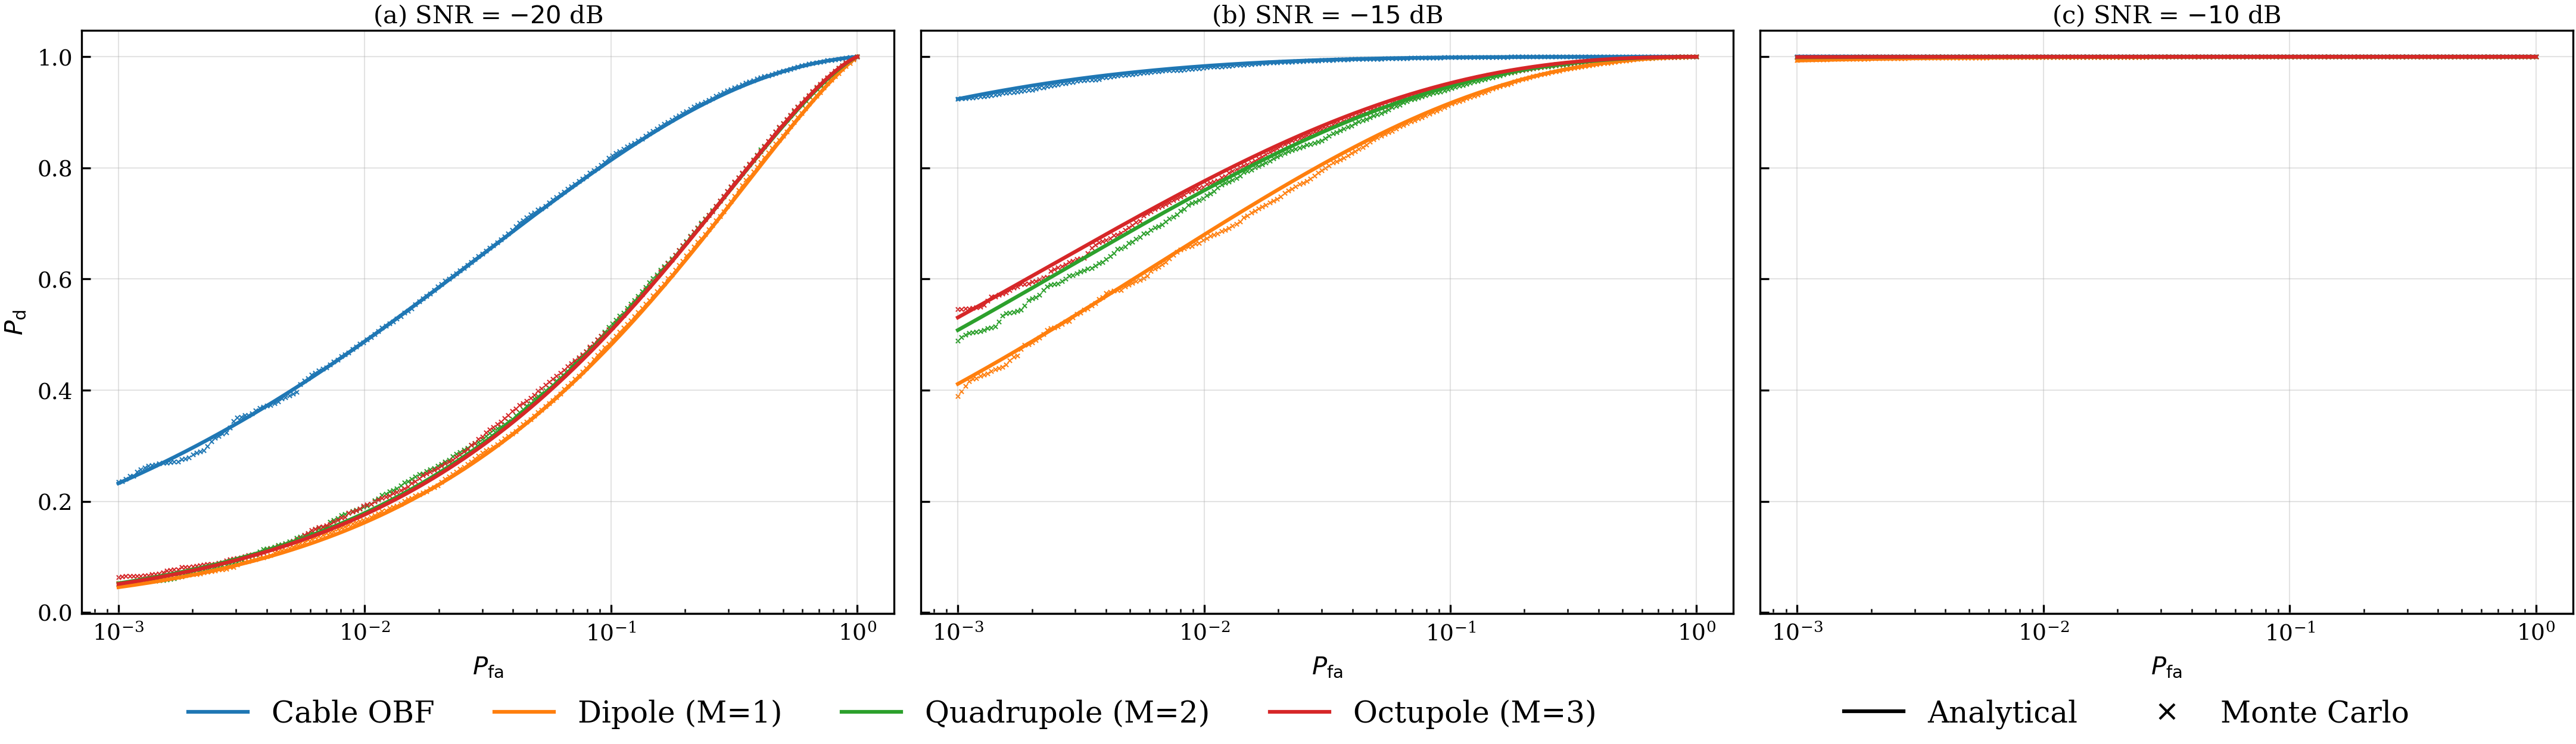
\includegraphics[width=1\textwidth]{results_and_discus/figures/ROCvsSNR.png}
    \caption{ROC curves for the cable OBF and MOBF receivers at several SNR levels obtained from the analytical form and by Monte Carlo simulation ($2\times10^4$ realizations).}
    \label{fig:ROCvsSNR}
\end{figure*}

\begin{figure}
    \centering
    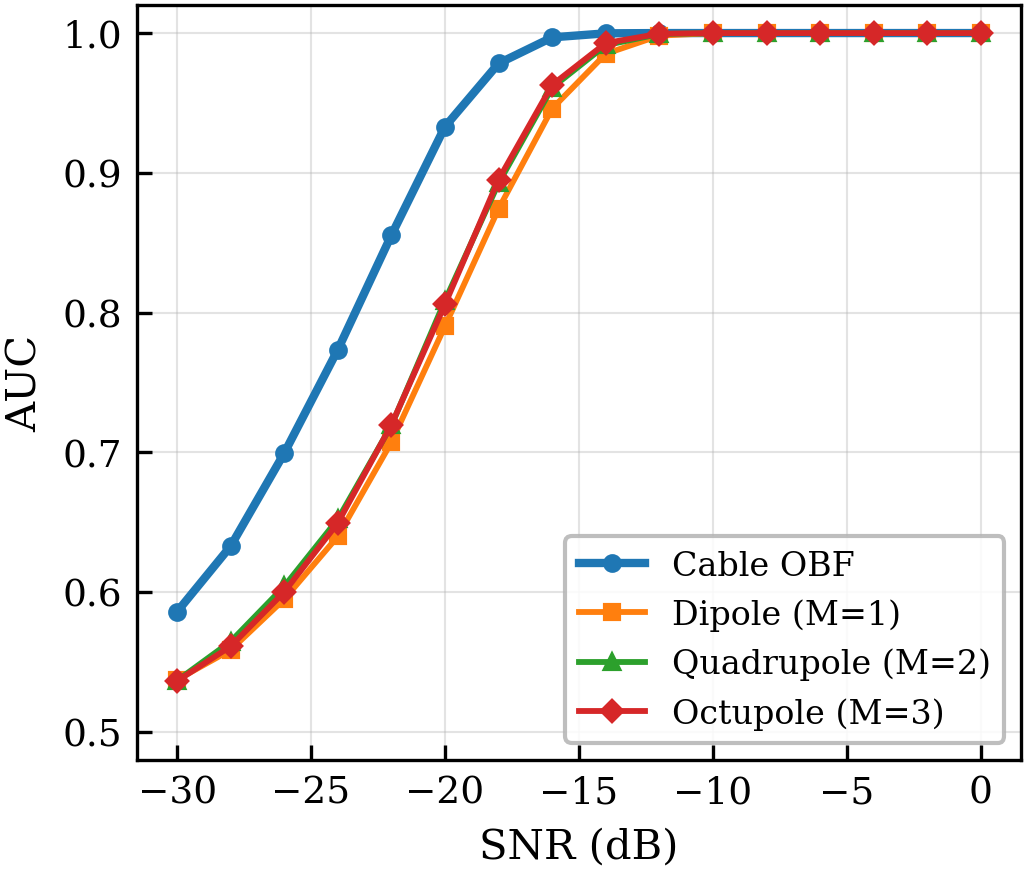
\includegraphics[width=\linewidth]{results_and_discus/figures/AUCvsSNR.png}
    \caption{Area under the ROC curve (AUC) as a function of SNR for the cable OBF and MOBF receivers of orders 1 to 3.}
    \label{fig:AUCvsSNR}
\end{figure}

Disregarding the detection offset discussed in section~\ref{sec:simulation}, the results here indicate that the MOBF is capable of detecting the cable. However, they also show that the matched cable OBF consistently outperforms or matched all considered MOBF orders, with the performance gap becoming particularly pronounced at SNR values below \(-15\)~dB. This behavior is attributable to the fact that the cable OBF captures the full energy of the signal \(s\) while involving the minimum number of noisy channels.

Finally, the behavior observed in Figure~\ref{fig:AUCvsSNR} is reproduced in Figure~\ref{fig:paramJumble} for different combinations of \(\psi\) and \(\delta\), providing further evidence that the cable OBF outperforms the MOBF for cable detection.


\begin{figure}
    \centering
    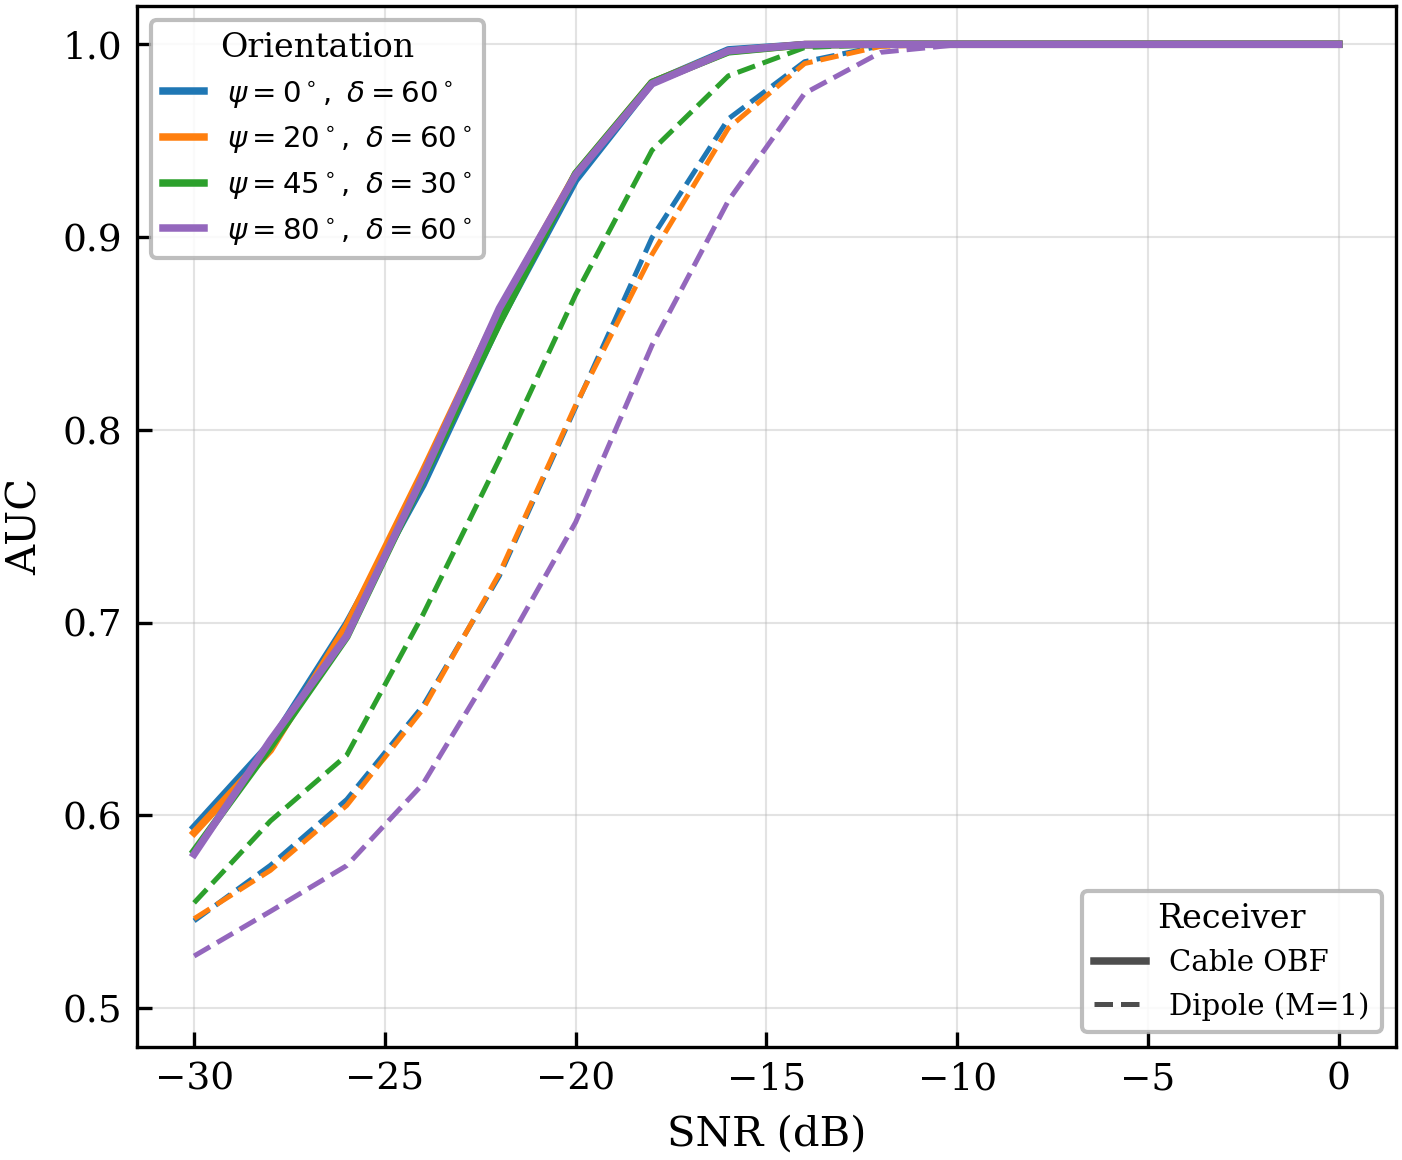
\includegraphics[width=\linewidth]{results_and_discus/figures/params_jumble.png}
    \caption{AUC as a function of SNR for varying orientation parameters $\psi$ and $\delta$ confirming that the cable OBF consistently outperforms MOBF receivers across orientations.}
    \label{fig:paramJumble}
\end{figure}